\documentclass[xcolor=dvipsnames]{beamer}
\useoutertheme{infolines}
\setbeamertemplate{navigation symbols}{}
\setbeamertemplate{items}[ball]
\usepackage{graphicx}
\usepackage{color}
\usepackage{xcolor}
\usepackage{verbatim}
\usepackage{float}
\setbeamertemplate{frametitle}[default][center]
\begin{document}
\title{Efficient methods for identifying mutated driver pathways in cancer}
\author{Bowen Deng}
\institute{Dept. of Prob. and Stat.}
\date{}
\begin{frame}
\maketitle
\end{frame}
\begin{frame}
Topics: The study in {\em Efficient methods for identifying mutated driver pathways in cancer} and my extension work.\\
\begin{itemize}
\item Motivation\\
\item Studies Ad hoc\\
\item Studies in the paper\\
\item Potential Improvement\\
\item My Studies\\
\item Further Challenges
\end{itemize}
\end{frame}
\section{Motivation}
\subsection{Biological Issue}
\begin{frame}{Identifying Driver mutations}
Cancer is driven by somatic mutations in the genome, including single nucleotide mutations and larger copy-number aberrations and structural aberrations.\\
With the availability of NGS technologies, whole-genome or whole-exome measurements of the somatic mutations in large numbers of cancer genomes are now a reality.\\
A major challenge for these studies is to distinguish the functional 'driver mutations' responsible for cancer from the random 'passenger mutations' that have accumulated in somatic cells but that are not important for cancer development.\\
\end{frame}
\section{Studies Ad hoc}
\begin{frame}{Preliminary Studies}
A standard approach to predict driver mutations is to identify recurrent mutations in a large cohort of cancer patients.\\
This approach has identified several important cancer mutations (e.g., in KRAS, BRAF, ERRB2, etc.), but has not revealed all of the driver mutations in individual cancers.\\
Rather, the results from initial studies have confirmed that cancer genomes exhibit extensive mutational heterogeneity with no two genomes-even those from the same tumor type-containing exactly the same complement of somatic mutations.\\
This heterogeneity results from the presence of passenger mutations in each cancer genome and because driver mutations often targets genes in cellular signaling and regulatory pathways.\\
\end{frame}
\begin{frame}{Pathway Level Studies}
Since each of these pathways contains multiple genes, there are numerous combinations of driver mutations that can perturb a pathway important for cancer.\\
This mutational heterogeneity complicates efforts to identify functional mutations by their recurrence across many samples, as the number of patients required to demonstrate recurrence of rare mutations is very large.\\
Most recent cancer genome sequencing papers analyze known pathways for enrichment of somatic mutations, and methods that identify known pathways that are significantly mutated across many patients have been developed.\\
In addition, algorithms that extend pathway analysis to genome-scale gene interaction networks have recently been introduced.\\
\end{frame}
\begin{frame}{Difficulties and Solutions}
While some pathways are well-characterized and cataloged in various databases, knowledge of pathways remains incomplete.\\
These concerns, plus the availability of increasing numbers of sequenced cancer genomes, motivate the question of whether it is possible to discover groups of genes with driver mutations automatically directly from somatic mutation data collected from large numbers of patients.\\
De novo discovery of mutated driver pathways seems implausible because of the enormous number of possible gene sets to test: e.g., there are more than $10^{26}$ sets of seven human genes.\\
However, the current understanding of the somatic mutational process of cancer places two additional constraints on the expected patterns of somatic mutations that significantly reduce the number of gene sets to consider.\\
\end{frame}
\subsection{Coverage Principle}
\begin{frame}{Coverage Principle}
An important cancer pathway should be perturbed in a large number of patients.\\
Thus, given genome-wide measurements of somatic mutations, we expect that most patients will have a mutation in some gene in the pathway.
\end{frame}
\subsection{Exclusivity Principle}
\begin{frame}{Exclusivity Principle}
A driver mutation in a single gene of the pathway is often assumed to be sufficient to perturb the pathway.\\
Combined with the fact that driver mutations are relatively rare, most patients exhibit only a single driver mutation in a pathway.\\
\end{frame}
\begin{frame}{Selective Advantage}
Tumorigenesis is a consequence of a series of mutations, which can be viewed as an annually accumulated Darwinian evolutionary process.\\
Mutations of two genes participating in the same pathway or process rarely confer a significant selective advantage compared to the single mutation, since the functional consequences of single and double mutations are similar.\\
By contrast, functional consequences of mutations of multiple genes that participate in different pathways or functions may be additive or even synergistic in conferring an advantage to the tumor. Therefore, we would expect to observe a tendency of mutually exclusive mutations of genes in the same pathway and the tendency of co-occurring mutations of genes that populated distinct pathways.\\
\end{frame}
\begin{frame}{Illustration}
Take as instance the following graph, if we infect two genes and let the cancer cells proliferate via the network.\\
When we infect NOTCH1 and CDKN2A which are in the same pathway, the result would be the infection of the whole pathway and those genes related with the pathway.\\
\begin{figure}
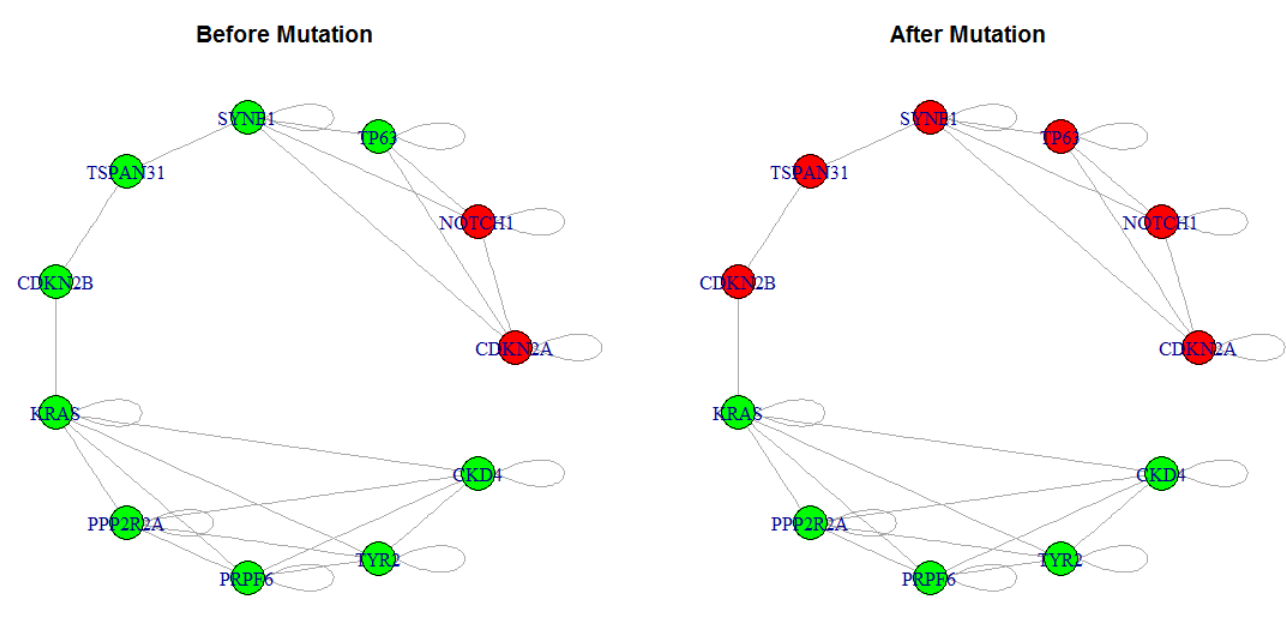
\includegraphics[width=0.9\linewidth]{BeforeMutation1.png}
\end{figure}
\end{frame}
\begin{frame}{Illustration}
On the other hand, if we infect CDKN2A and TYR2 that are in different pathways, both pathways and their neighbors are infected.\\
The result of infecting genes in different pathways is more far-reaching and disastrous. The infectors should fit to live and infect efficiently by attacking more pathways rather than more genes in the same pathway.
\begin{figure}
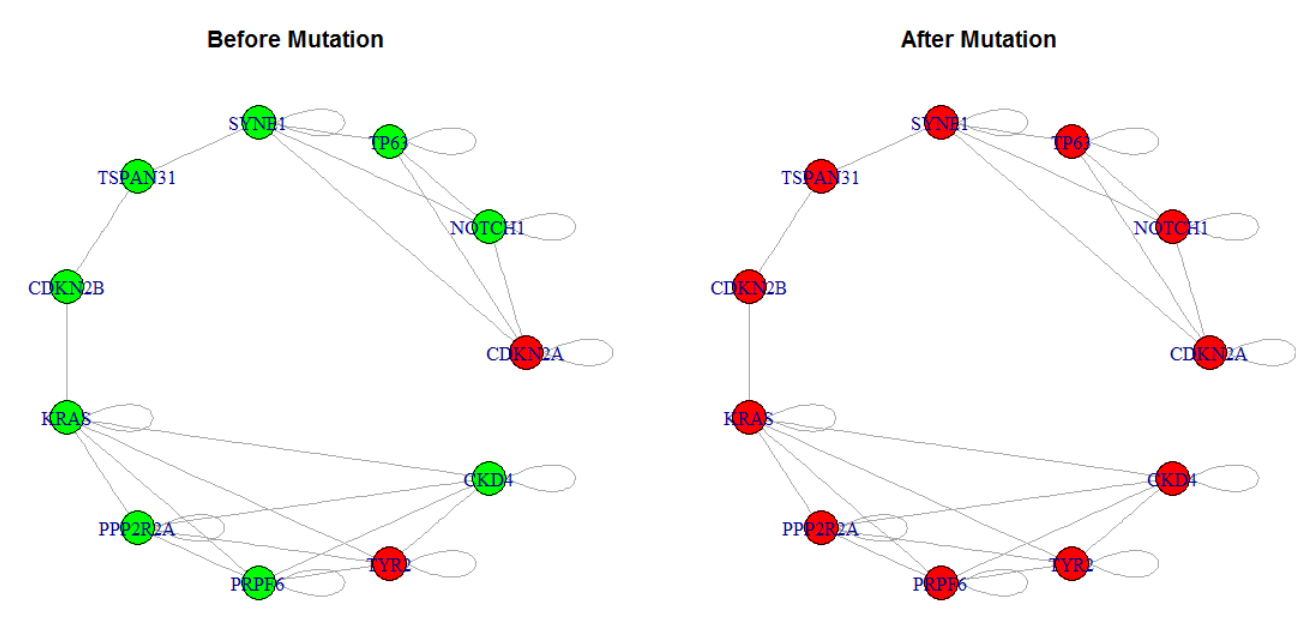
\includegraphics[width=0.9\linewidth]{BeforeMutation2.png}
\end{figure}
\end{frame}
\begin{frame}{Supporting Evidence}
There are numerous example of pairs of mutually exclusive driver mutations including EGFR and KRAS mutations in lung cancer, TP53 and MDM2 mutations in glioblastoma et al., and KRAS and PTEN mutations in endometrial and skin cancers.
\end{frame}
\subsection{Mathematical Translation}
\begin{frame}{Mutation Matrix}
Consider mutation data for $m$ cancer patients, where each of $n$ genes is tested for a somatic mutation in each patient.\\
We represent the mutation data by a mutation matrix A with $m$ rows and $n$ columns, where each row is a patient and each column is a gene.\\
The entry $A_{ij}$ in row $i$ and column $j$ is equal to 1 if gene $j$ is mutated in patient $i$, and it is 0 otherwise.\\
For a gene $g$, let $\Gamma(g)=\{i:A_{ig}=1\}$ denote the sets of patients in which $g$ is mutated.\\
Similarly, for a set $M$ of genes, let $\Gamma(M)$ denote the set of patients in which at least one of the genes in $M$ is mutated: $\Gamma(M)=\cup_{g\in M}\Gamma(g)$.\\
\end{frame}
\begin{frame}
Earlier studies employed straightforward statistical tests to test for exclusivity between pairs of genes.\\
More sophisticated tests for pairwise exclusivity have also been proposed.\\
However, it is not clear how to extend such pairwise tests to larger groups of genes, particularly because the number of hypotheses grows rapidly as the number of genes in the set increases.\\
\end{frame}
\begin{frame}{Intransitivity}
Moreover, identification of pairs of mutually exclusive mutated genes is not sufficient for identification of larger sets, since mutual exclusion relations are not transitive.\\
For example, consider two patients $s_1$ and $s_2$: In $s_1$, only gene $x$ is mutated; in $s_2$, genes $(y,z)$ are mutated.\\
The pairs of genes $(x,y)$ and $(x,z)$ are mutually exclusive, but the pair $(y,z)$ is not.\\
\begin{figure}
\centering
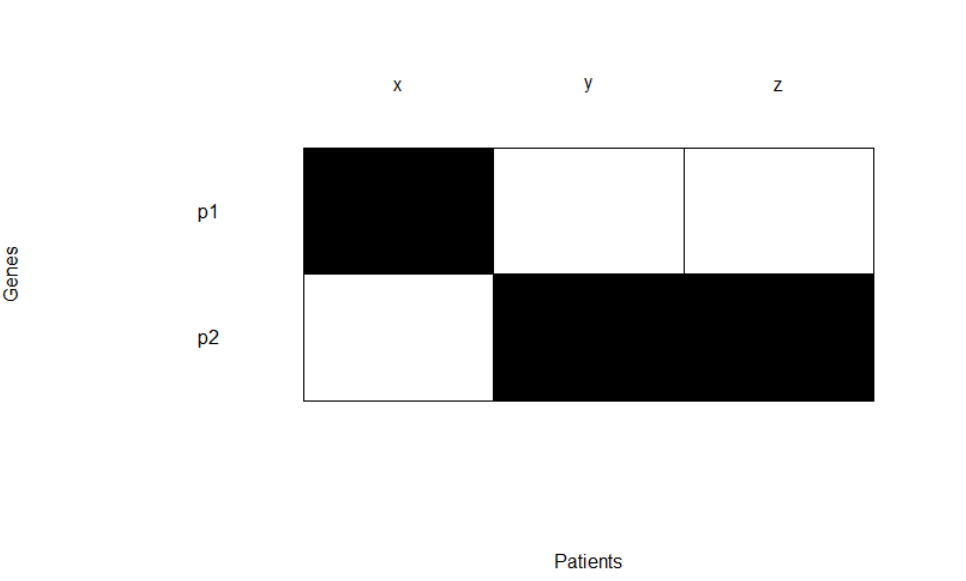
\includegraphics[width=0.6\linewidth]{pg.png}
\end{figure}
\end{frame}
\begin{frame}
Finding the largest set of genes with mutually exclusive mutations is NP-hard by reduction from maximum independent set.\\
Instead, we propose to identify sets of genes (columns of the mutation matrix) that are mutated in a large number of patients and whose mutations are mutually exclusive.\\
\textbf{Maximum Coverage Exclusive Submatrix Problem:} Given an $m\times n$ mutation matrix $A$ and an integer $k>0$, find a mutually exclusive $m\times k$ submatrix $M$ of $k$ columns (genes) of $A$ with the largest number of nonzero rows (patients).\\
\end{frame}
\begin{frame}
We do not expect mutations in driver pathways to be mutually exclusive because of measurement errors and the presence of passenger mutations.\\
Instead, we aim to find a set $M$ of genes that satisfies the following two requirements:\\
1. {\em Coverage:} Most patients have at least one mutation in $M$.\\
2. {\em Approximate exclusivity:} Most patients have no more than one mutation in $M$.\\
There is an obvious trade-off between requiring mutual exclusivity in the set and obtaining low coverage versus allowing greater non-exclusivity in the set and obtaining larger coverage.\\
\end{frame}
\begin{frame}
We introduce a measure on a set of genes that quantities the tradeoff between coverage and exclusivity.\\
For a set $M$ of genes, we define the coverage overlap\\
\[
\omega(M)=\sum_{g\in M}|\Gamma(g)|-|\Gamma(M)|.
\]
Note that $\omega(M)\geqslant 0$ with equality holding when the mutations in $M$ are mutually exclusive.\\
To take into account both the coverage $\Gamma(M)$ and the coverage overlap $\omega(M)$ of $M$, we define the weight\\
\[
W(M)=|\Gamma(M)|-\omega(M)=2|\Gamma(M)|-\sum_{g\in M}|\Gamma(g)|.
\]
Note that the weight function $W(M)$ is only one possible measure of the trade-off between coverage and exclusivity.
\end{frame}
\begin{frame}{MWSP}
\textbf{Maximum Weight Submatrix Problem (MWSP):} Given an $m \times n$ mutation matrix A and an integer $k > 0$, find the $m \times k$ column submatrix $\hat{M}$ of A that maximizes W(M).\\
In the studies ad hoc, Vandin et al. proposed a greedy algorithm and an Metropolis-Hasting algorithm to solve the MWSP.\\
\begin{figure}
\centering
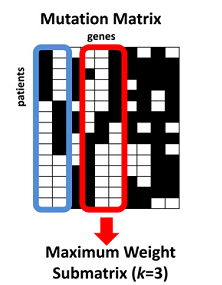
\includegraphics[width=0.3\linewidth]{mat.png}
\end{figure}
\end{frame}
\section{Studies in the paper}
\subsection{BLP Model}
\begin{frame}{BLP Model}
The first innovation of the paper is to translate the original combinatorial optimization problem, i.e. finding an $m\times k$ submatrix $M$ in the $m\times n$ matrix $A$ with the maximum $W(M)$ into an IP:\\
\begin{eqnarray}
\max F(x,y)=2\sum_{i=1}^my_i-\sum_{j=1}^n(x_j\cdot\sum_{i=1}^ma_{ij})\nonumber\\
s.t.
\left\{
\begin{array}{c}
\sum_{j=1}^na_{ij}x_j\geqslant y_i, i=1,\cdots,m\\
\sum_{j=1}^nx_j=k,\\
y_i,x_j\in\{0,1\},i=1,\cdots,m,j=1,\cdots,n.
\end{array}
\right.\nonumber
\end{eqnarray}
where $x_j$ is the indicator whether column $j$ of $A$ falls into the submatrix $M$, $y_i$ is the indicator whether the entries of row $i$ of $M$ are not all zeros.\\
\end{frame}
\begin{frame}{Algorithms}
To solve the MWSP, the authors of the paper applied the Branching and Bounding algorithm (BB algorithm) and Genetic Algorithm (GA).\\
\end{frame}
\subsection{Integrated Mutation and gene Expression data}
\begin{frame}
In real applications, there may be multiple optimal solutions. Moreover, due to the noise in the data or other factors, the most optimal ones may not be the best one in biological context.\\
To extract the most biologically significant ones, we generalize the above model by integrating the gene expression data to improve its performance.\\
Our new model is based on such as observation that the genes in the same pathway usually collaborate with each other to execute one function.\\
Therefore, the expression profile of gene pairs in the same pathway usually have higher correlations than that in different pathways.\\
\end{frame}
\begin{frame}
We can use this characteristic to discriminate the gene sets with the same score.\\
Besides, to filter out the noise in the data and detect more meaningful gene sets, we try to identify such gene sets, whose scores $W(M)$ are close to the optimal solution, but whose member genes have higher correlations with each other.\\
\begin{figure}
\centering
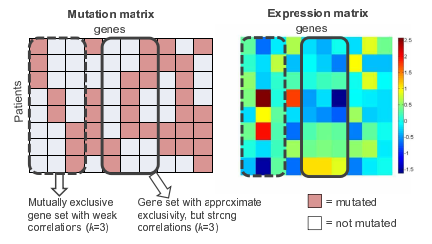
\includegraphics[width=0.6\linewidth]{express.png}
\end{figure}
\end{frame}
\begin{frame}
By combining the gene expression data with the earlier problem, we define the following new measure:
\[
F_{ME}=W(M)+\lambda R(E_M)
\]
where $R(E_M)=\sum_{j_1\neq j_2}\frac{|\text{pcc}(x_{j_1},x_{j_2})|}{\frac{k(k-1)}{2}}$, $E_M$ is the gene expression submatrix which corresponds to the same gene set with the mutation submatrix $M$, $\text{pcc}(\cdot)$ is the Pearson correlation coefficient, and $x_{j_1}$ and $x_{j_2}$ are the expression profiles of gene $j_1$ and $j_2$ in $E_M$ respectively.\\
Although the maximization of $F_{ME}$ can be formulated into a binary quadratic programming problem, it is limited by the computational complexity. Here we adopt the GA framework to solve it similarly.
\end{frame}
\section{Potential Improvements}
\begin{frame}{Potential Improvements}
The coverage principle of the driver pathway is definitely reasonable. Yet, the exclusivity principle deduced from natural selection is not widely accepted.\\
Therefore, we should build a flexible model for tradeoff between coverage and exclusivity.\\
A natural one would be imposing a tuning parameter in the original model.\\
\end{frame}
\section{My studies}
\begin{frame}{Weighted Sum of Row Scores}
Mathematically, we want to solve the following problem:\\
Maximum Weighted Sum of Row Scores Problem (MaWeSRoS): For an adjustable scoring function $s(x),x\in \mathbb{Z}^+\cup \{0\}$, and assuming $s$ gets its maximum at $x=1$,  we want to find an $m\times k$ submatrix $M$ in $m\times n$ mutation matrix $A$, such that it maximize the scoring function:
\[
S(M)=\sum_{i=1}^nw_is(r_i)
\]
where $r_i$ is the $i-th$ row sum in $M$, $w_i$ is the weight of the $i-th$ row, we take $w_i$ be the sum of the $i-th$ row.\\
\end{frame}
\begin{frame}{BLP Equivalence}
My model could be considered as the following BLP model:
\begin{eqnarray}
\max F(x)=2\sum_{i=1}^mw_is(\sum_{j=1}^nx_ja_{ij})\nonumber\\
s.t.
\left\{
\begin{array}{c}
\sum_{j=1}^nx_j=k,\\
x_i\in\{0,1\},i=1,\cdots,n.
\end{array}
\right.\nonumber
\end{eqnarray}
where $x_j$ is the indicator whether column $j$ of $A$ falls into the submatrix $M$, $y_i$ is the indicator whether the entries of row $i$ of $M$ are not all zeros.\\
\end{frame}
\begin{frame}{Relation with MWSP}
Moreover, MaWeSRoS is compatible for the integrative model in the paper. Just consider maximization of
\[
S(M)+\lambda R(E_M).
\]
For the original MWSP, $s(x)=1-|x-1|$, so MaWeSRoS has included the original MWSP.\\
\end{frame}
\begin{frame}{Different Score Functions}
Denote $s(x)=1-p(|x-1|)$, we can apply different $p(\cdot)$: $p_1(x)=\sqrt{x}$ for more emphasis on coverage, $p_2(x)=x^2$ for more emphasis on exclusivity. We can also set asymmetric scores. For example, we could apply different scores for different types of cancers according to our prior knowledge on it.\\
\begin{figure}
\centering
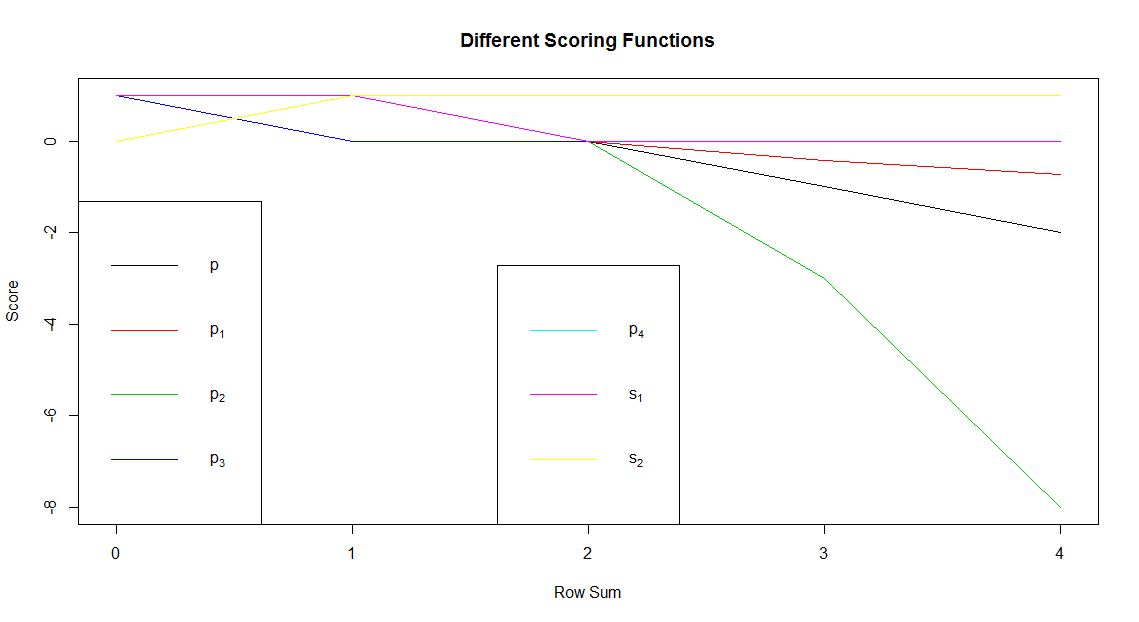
\includegraphics[width=0.8\linewidth]{diffscores.png}
\end{figure}
\end{frame}
\begin{frame}
Under this framework, the difficulty of the original BLP problem could be understood. $s(x)=1-|x-1|$ has a sharp point at $x=1$, thus it needs other constraints to describe $s(0)$, doubling the variables. Therefore, we could use square penalty, but the problem is also expensive since it is a quadratic programming (QP) problem. And square root penalty will make it harder.\\
Therefore, a general algorithm concerning this model is in need and it is not easy.\\
\end{frame}
\begin{frame}
As we know, the combinatorial optimization problem is NP-hard. Therefore, we would like to reduce the computational cost by relaxing the binary condition. The original problem became a restricted optimization problem.\\
\begin{eqnarray}
\max F(x)=2\sum_{i=1}^mw_is(\sum_{j=1}^nx_ja_{ij})\nonumber\\
s.t.
\left\{
\begin{array}{c}
\sum_{j=1}^nx_j=k,\\
0\leqslant x_i\leqslant1,i=1,\cdots,n.
\end{array}
\right.\nonumber
\end{eqnarray}
\end{frame}
\subsection{Simulation Study}
\begin{frame}{Generation of Data}
We simulated mutation data starting with gene sets $M_1,M_2,\cdots,M_I (I\geqslant 1)$. Every set has $k$ genes ($k=10$ has been used in this study).\\
For each patient, we mutate a gene chosen uniformly at random in $M_i$ with probability $p_i=1-i\Delta(\Delta=0.05 \text{ was used in this study})$, and if a gene in $M_i$ is mutated, then with probability $p_0$ we mutate other genes in $M_i$ ($p_0=0.04$ was used in this study).\\
$p_i$ and $p_0$ control the coverage and exclusivity of $M$ respectively. The genes not in $M_i$ are mutated at most in three samples. The parameter $I$ controls the complexity of the data structure.\\
\end{frame}
\begin{frame}
We use GA for various scoring functions to check the accuracy of each scoring function. And take $I=1$, $k=10$, $m=500$, $n=200$. The mutation matrix is shown in the figure.\\
\begin{figure}
\centering
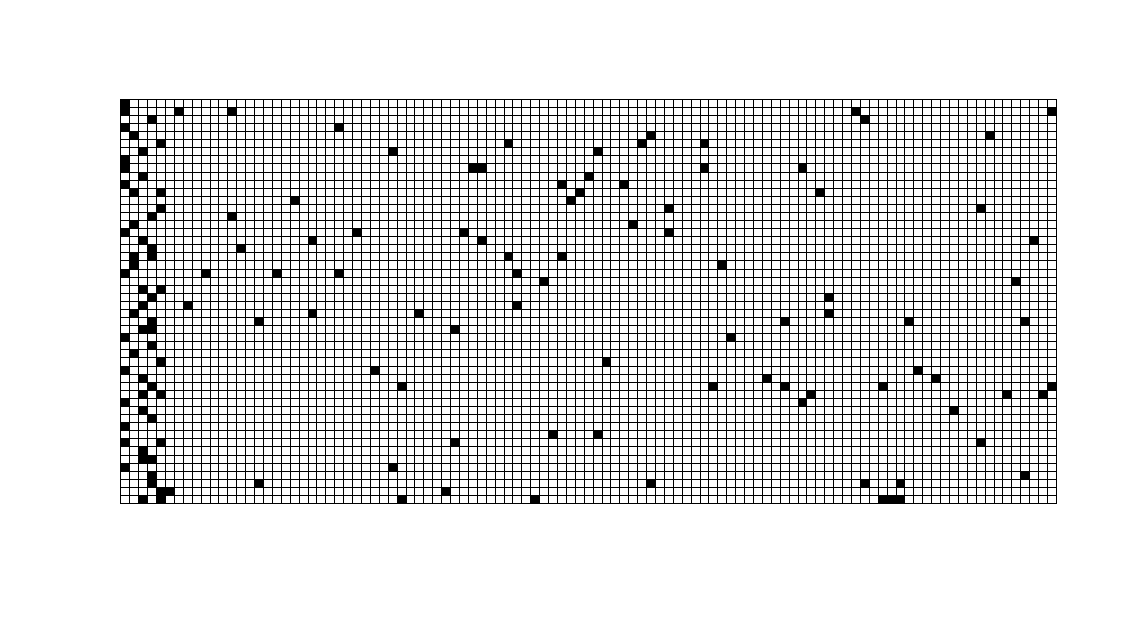
\includegraphics[width=0.8\linewidth]{simdata.png}
\end{figure}
\end{frame}
\begin{frame}
By theory, we should identify $1,2,\cdots,10$ as the pathway according to the data generation process. The result after 1000 iterations of Genetic Algorithm is shown in the table.\\
\begin{table}
\centering
\begin{tabular}{c|c|c|c}
\hline
$s(x)$&pathway&score&score of first 10 genes\\
\hline
$1-|1-x|$&  1   3   4   5   6 &41&30\\
(MWSP)& 9  10  32  81 106&&\\
$1-(1-x)^2$&1   5   6   7   9&43&28\\
(harsh penalty)&10  32  49  54 102&&\\
$1-\sqrt{1-x}$&1   5   6   7   9&43&30.58\\
(loose penalty)&10  32  47  54 102&&\\
\end{tabular}
\end{table}
\end{frame}
\begin{frame}
Fixing other parameters, set $I=1$.\\
\begin{figure}
\centering
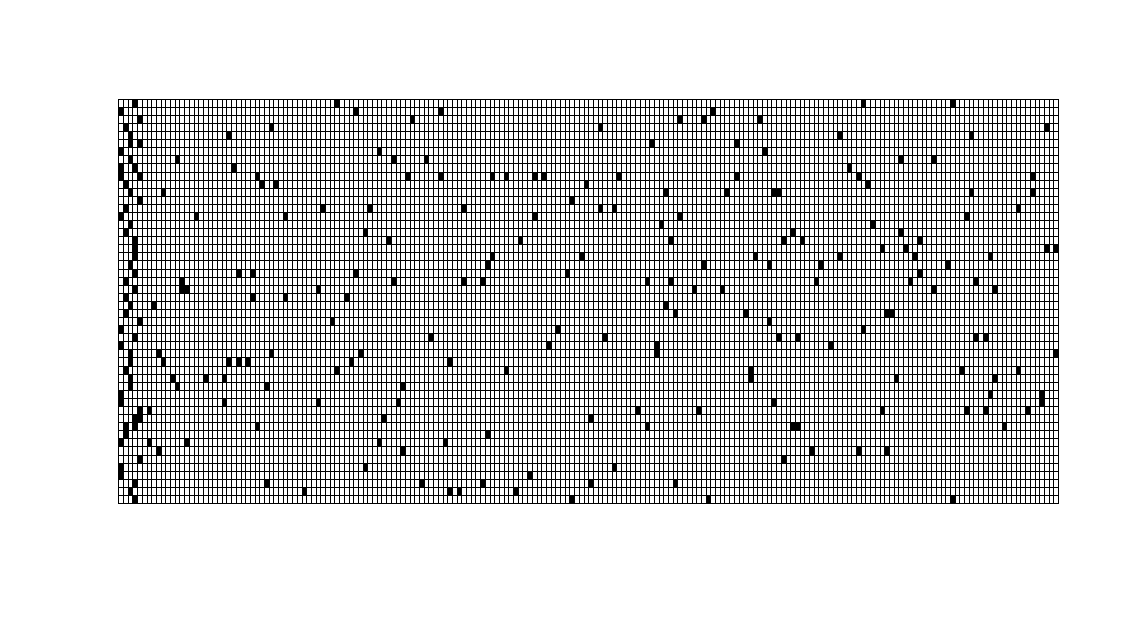
\includegraphics[width=0.8\linewidth]{recent.png}
\end{figure}
\end{frame}
\begin{frame}
Different from previous simulations, we only identify 5 genes.
\begin{table}
\centering
\begin{tabular}{c|c|c}
\hline
$s(x)$&pathway&score\\
\hline
MWSP&  1 2  3   4  5 &44\\
Harsh&1 2 3 4 5&44\\
Loose&1 2 3 4 37&41\\
\end{tabular}
\end{table}
\end{frame}
\begin{frame}
Fixing other parameters, set $k=5$.\\
\begin{figure}
\centering
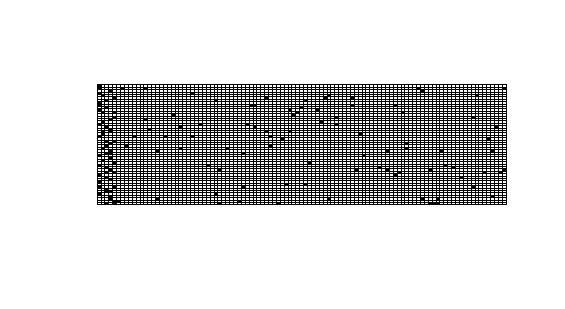
\includegraphics[width=0.8\linewidth]{newmut.png}
\end{figure}
\end{frame}
\begin{frame}
\begin{table}
\centering
\begin{tabular}{c|c|c|c}
\hline
$s(x)$&pathway&score&score of first 5 genes\\
\hline
$1-|1-x|$&  1 2  3   4  51 &41&39\\
$1-(1-x)^2$&1 2 3 4 49&41&39\\
$1-\sqrt{1-x}$&1 2 3 4 37&41&39\\
\end{tabular}
\end{table}
\end{frame}
\section{Further Challenges}
\begin{frame}{Challenges}
The challenges of the new framework are twofold:\\
\begin{itemize}
\item Which score function to use\\
\item How to solve the optimization problem efficiently\\
\item How to tune k\\
\end{itemize}
\end{frame}
\end{document}
